\chapter{Background}

\section{Wireless Communications}

This section aims to provide a general overview of wireless communication terminology and other principles needed to understand the more hardware-oriented part of this thesis.

\subsection{Problems with established wireless communication techniques}

\begin{figure}
    \centering
    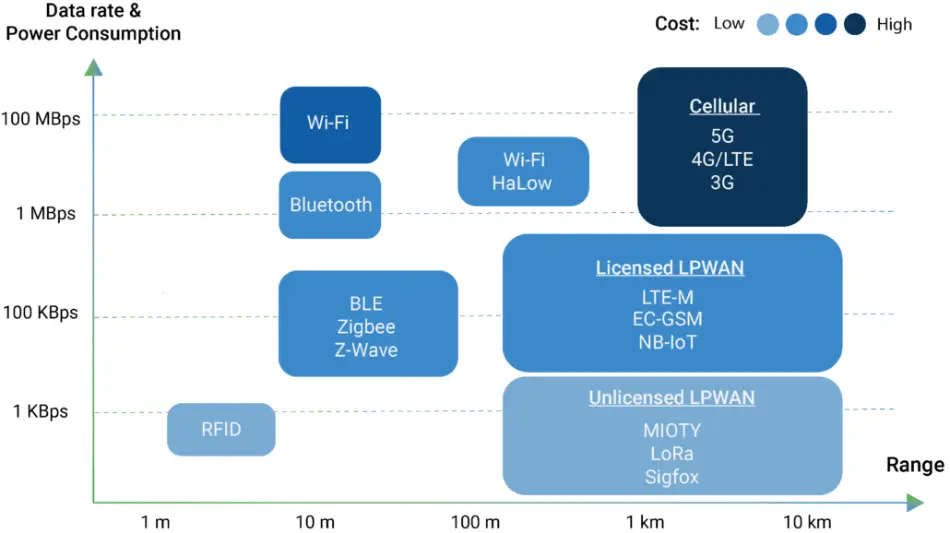
\includegraphics[width=1\textwidth]{pictures/lora/comparison-wireless-protocols.png}
    \caption{Comparison of data rate, power consumption and range between different wireless communication protocols~\protect\cite{wang_comparison_2021}}\label{pic:wireless-protocols-comparison}
\end{figure}

While there are sensors that can be connected to the internet using Wi-Fi, ZigBee, \ac{LTE} and other, these technologies are not suitable for all use cases.

Deployments in remote or particularly spacious areas might need long-range protocols.
Likewise, sensors that are deployed in such areas can be hard to reach or placed apart by several hundred meters.
This makes low-power sensors that need to run on batteries for several years a necessity since replacing the batteries can be expensive or even impossible.

Wi-Fi is not suitable for battery-powered devices that are deployed in remote areas, as it requires relatively high power to operate and doesn't have much range.
ZigBee is also not suitable for battery-powered devices, as it is not designed for long distances and thus has a short range.
\ac{LTE} not suitable for battery-powered devices either as it requires a lot of power.
A rough comparison between selected wireless protocols can be seen in \cref{pic:wireless-protocols-comparison}~\cite{wang_comparison_2021}.

\subsection{\acf{RSSI}}\label{sec:rssi}

The \acl{RSSI} is a measure of the strength of a signal received by a device.
As far as this thesis is concerned, \ac{RSSI} values are measured in dBm since \ac{TTN}, the basis for all data used, uses this unit as well~\cite{the_things_industries_bv_data_2023}.

% TODO: Quote for this? It's basically just physics?
Usually, the higher the \ac{RSSI} value, the closer the sender is to the receiver since the signal is stronger when the radio waves have to travel a shorter distance.
Different devices can have different \ac{RSSI} values for the same distance because of factors such as antennas with different gains.

\ac{RSSI} values can only function reliably when there is nothing blocking the signal between the transmitting and receiving stations, e.g.,\ if there is a line of sight between the sender and receiver.
The \ac{RF} signal can be blocked and thereby attenuated by walls, trees, or other objects.

\subsubsection{\acf{MPP}}\label{sec:multipath-propagation}

\begin{figure}
    \centering
    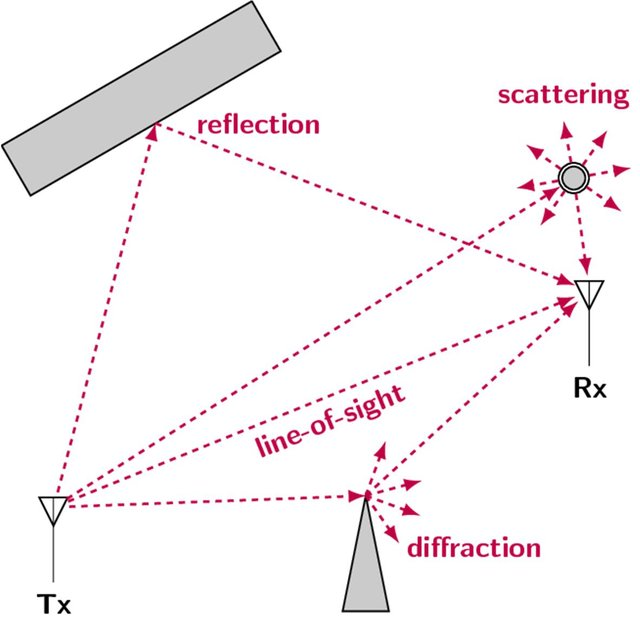
\includegraphics[width=0.4\textwidth]{pictures/diagrams_figures/multipath_propagation.jpg}
    \caption{Example for \acf{MPP} of \ac{RF} waves\protect\cite{milosevic_key_2017}}\label{pic:figure_multipath_propagation}
\end{figure}

Additionally, a \ac{RF} transmission phenomenon called \acf{MPP} can occur.
\acl{MPP} cause the \ac{RSSI} values to fluctuate even when neither the distance between the sender and receiver nor their antennas change~\cite[p. 136]{abdelfadeel_how_2019}.
This is because the signal can be reflected, diffracted, refracted and scattered and therefore take several paths (hence the term \ac{MPP}) as can be seen in \cref{pic:figure_multipath_propagation}.

\subsection{\acf{SNR}}

The \acf{SNR} is a measure of the strength of the signal compared to the noise in the signal.
Its formula is as follows:

\begin{equation}
    \text{SNR} = \frac{P_{signal}}{P_{noise}}
\end{equation}

A low \ac{SNR} indicates a signal that is influenced by a lot of noise.
The \ac{SNR} can be impacted by several environmental factors, such as the temperature and humidity of the air~\cite{jeftenic_impact_2020}.

As far as this thesis is concerned, \ac{SNR} values were used alongside \ac{RSSI} values in fingerprinting.

\section{Terminology: \acs{LoRa} vs. \acs{LoRaWAN}}

\ac{LoRa} is a \ac{RF} communication modulation that offers a standard to send data packets over the air in a specific way.
The term \ac{LoRa} stands for \textbf{Lo}ng \textbf{Ra}nge~\cite{semtech_corporation_lora_2023}.
A rough explanation of its technical details can be found in \cref{sec:lora-modulation}.

\ac{LoRaWAN} is a network protocol that uses \ac{LoRa} as its physical layer.
It will be explained in more detail in \cref{sec:lorawan}.

\section{\acf{LoRa} modulation}\label{sec:lora-modulation}

% explain the basics of LoRa with things like modulation (Chirp Spread Spectrum), spreading factor, bandwidth, coding rate, channels etc.
While, in the 868 MHz band used in the \ac{EU}, there are only a few channels available, \ac{LoRa} uses a technique called modulation to overcome this problem.

\subsection{Chirp Spread Spectrum}

\ac{LoRa} uses a technique called \ac{CSS} to transmit data with the possibility for error detection and correction.

% TODO

\subsection{\acfp{SF}}\label{sec:spreading-factors}

The \ac{LoRa} modulation uses different \acp{SF} to transmit data.

% TODO explain spreading factors, their effect on data rate and range and their relevance for this thesis
% spreading factors: SF7 = high data rate, low range; SF12 = low data rate, high range

\subsubsection{Correlation of \acs{SF} and \acs{RSSI} + \acs{SNR}}

\subsection{Duty Cycle (in the \acs{EU} region)}

\begin{figure}
    \centering
    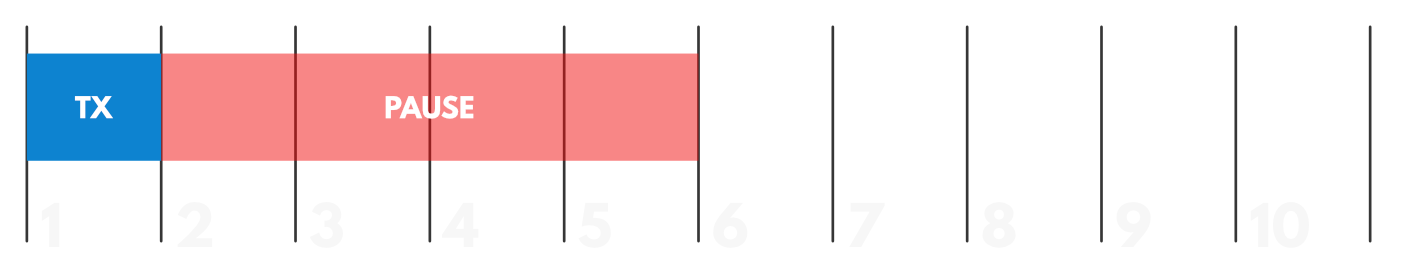
\includegraphics[width=.8\textwidth]{pictures/lora/duty-cycle-single-channel-off-air.png}
    \caption{\ac{LoRa} duty cycle example~\protect\cite{the_things_industries_bv_duty_nodate}}\label{pic:lora-duty-cycle}
\end{figure}

In the \ac{EU} region, the duty cycle for transmissions in the 868 MHz band is limited to 1\%~\cite{etsi_etsi_2012}.
This means that a \ac{LoRa} device using a frequency band in this range may only transmit for 1\% of a given time slot.
If, for example, a device transmits data for 36 seconds, it must stay silent for the following 3,564 seconds, which is almost an hour.
It needs to stay silent for the rest of the time.

An example of a \ac{LoRa} duty cycle can be seen in \cref{pic:lora-duty-cycle}.
In this example, the duty cycle is 20\%.
The device, which transmits for one block of time needs to stay silent for the next four blocks of time until it can transmit again.

Luckily, LoRa packets are usually only a few bytes small and can thus be transmitted in a short amount of time, usually in a few milliseconds.

\subsubsection{\ac{LoRa} transmission bit rates}

%  Explain how bit rates are affected by the duty cycle, spreading factor, bandwidth and coding rate

\subsection{Why use \acs{LoRa}?}

As can be seen in \cref{pic:wireless-protocols-comparison}, \ac{LoRa} is a good choice for devices that need to be able to operate battery-powered in remote locations for extended periods of time, as it has a long range and low power consumption.

A \ac{LoRa} node that transmits 75 bytes of payload data every 2 hours can theoretically last up to 10 years on a single 1000 mAh battery~\cite{cheong_comparison_2017-1}.
LoRa Energy Calculator\footnote{https://dramco.be/tools/lora-calculator/} is another piece of software that can be used to calculate the battery life of a \ac{LoRa} device by entering data such as payload size, periodicity of the data transmission and the battery type used.

\section{\acf{LoRaWAN}}\label{sec:lorawan}

\begin{figure}
    \centering
    
\includegraphics[width=.4\textwidth]{pictures/logos/LoRaWAN_Logo.eps}
    \caption{\ac{LoRaWAN} logo~\protect\cite{lora_alliance_francais_2022}}
\end{figure}

\ac{LoRaWAN} uses the LoRa wireless communication protocol to create a \ac{WAN} where multiple devices can communicate with each other over long distances.

\begin{figure}
    \centering
    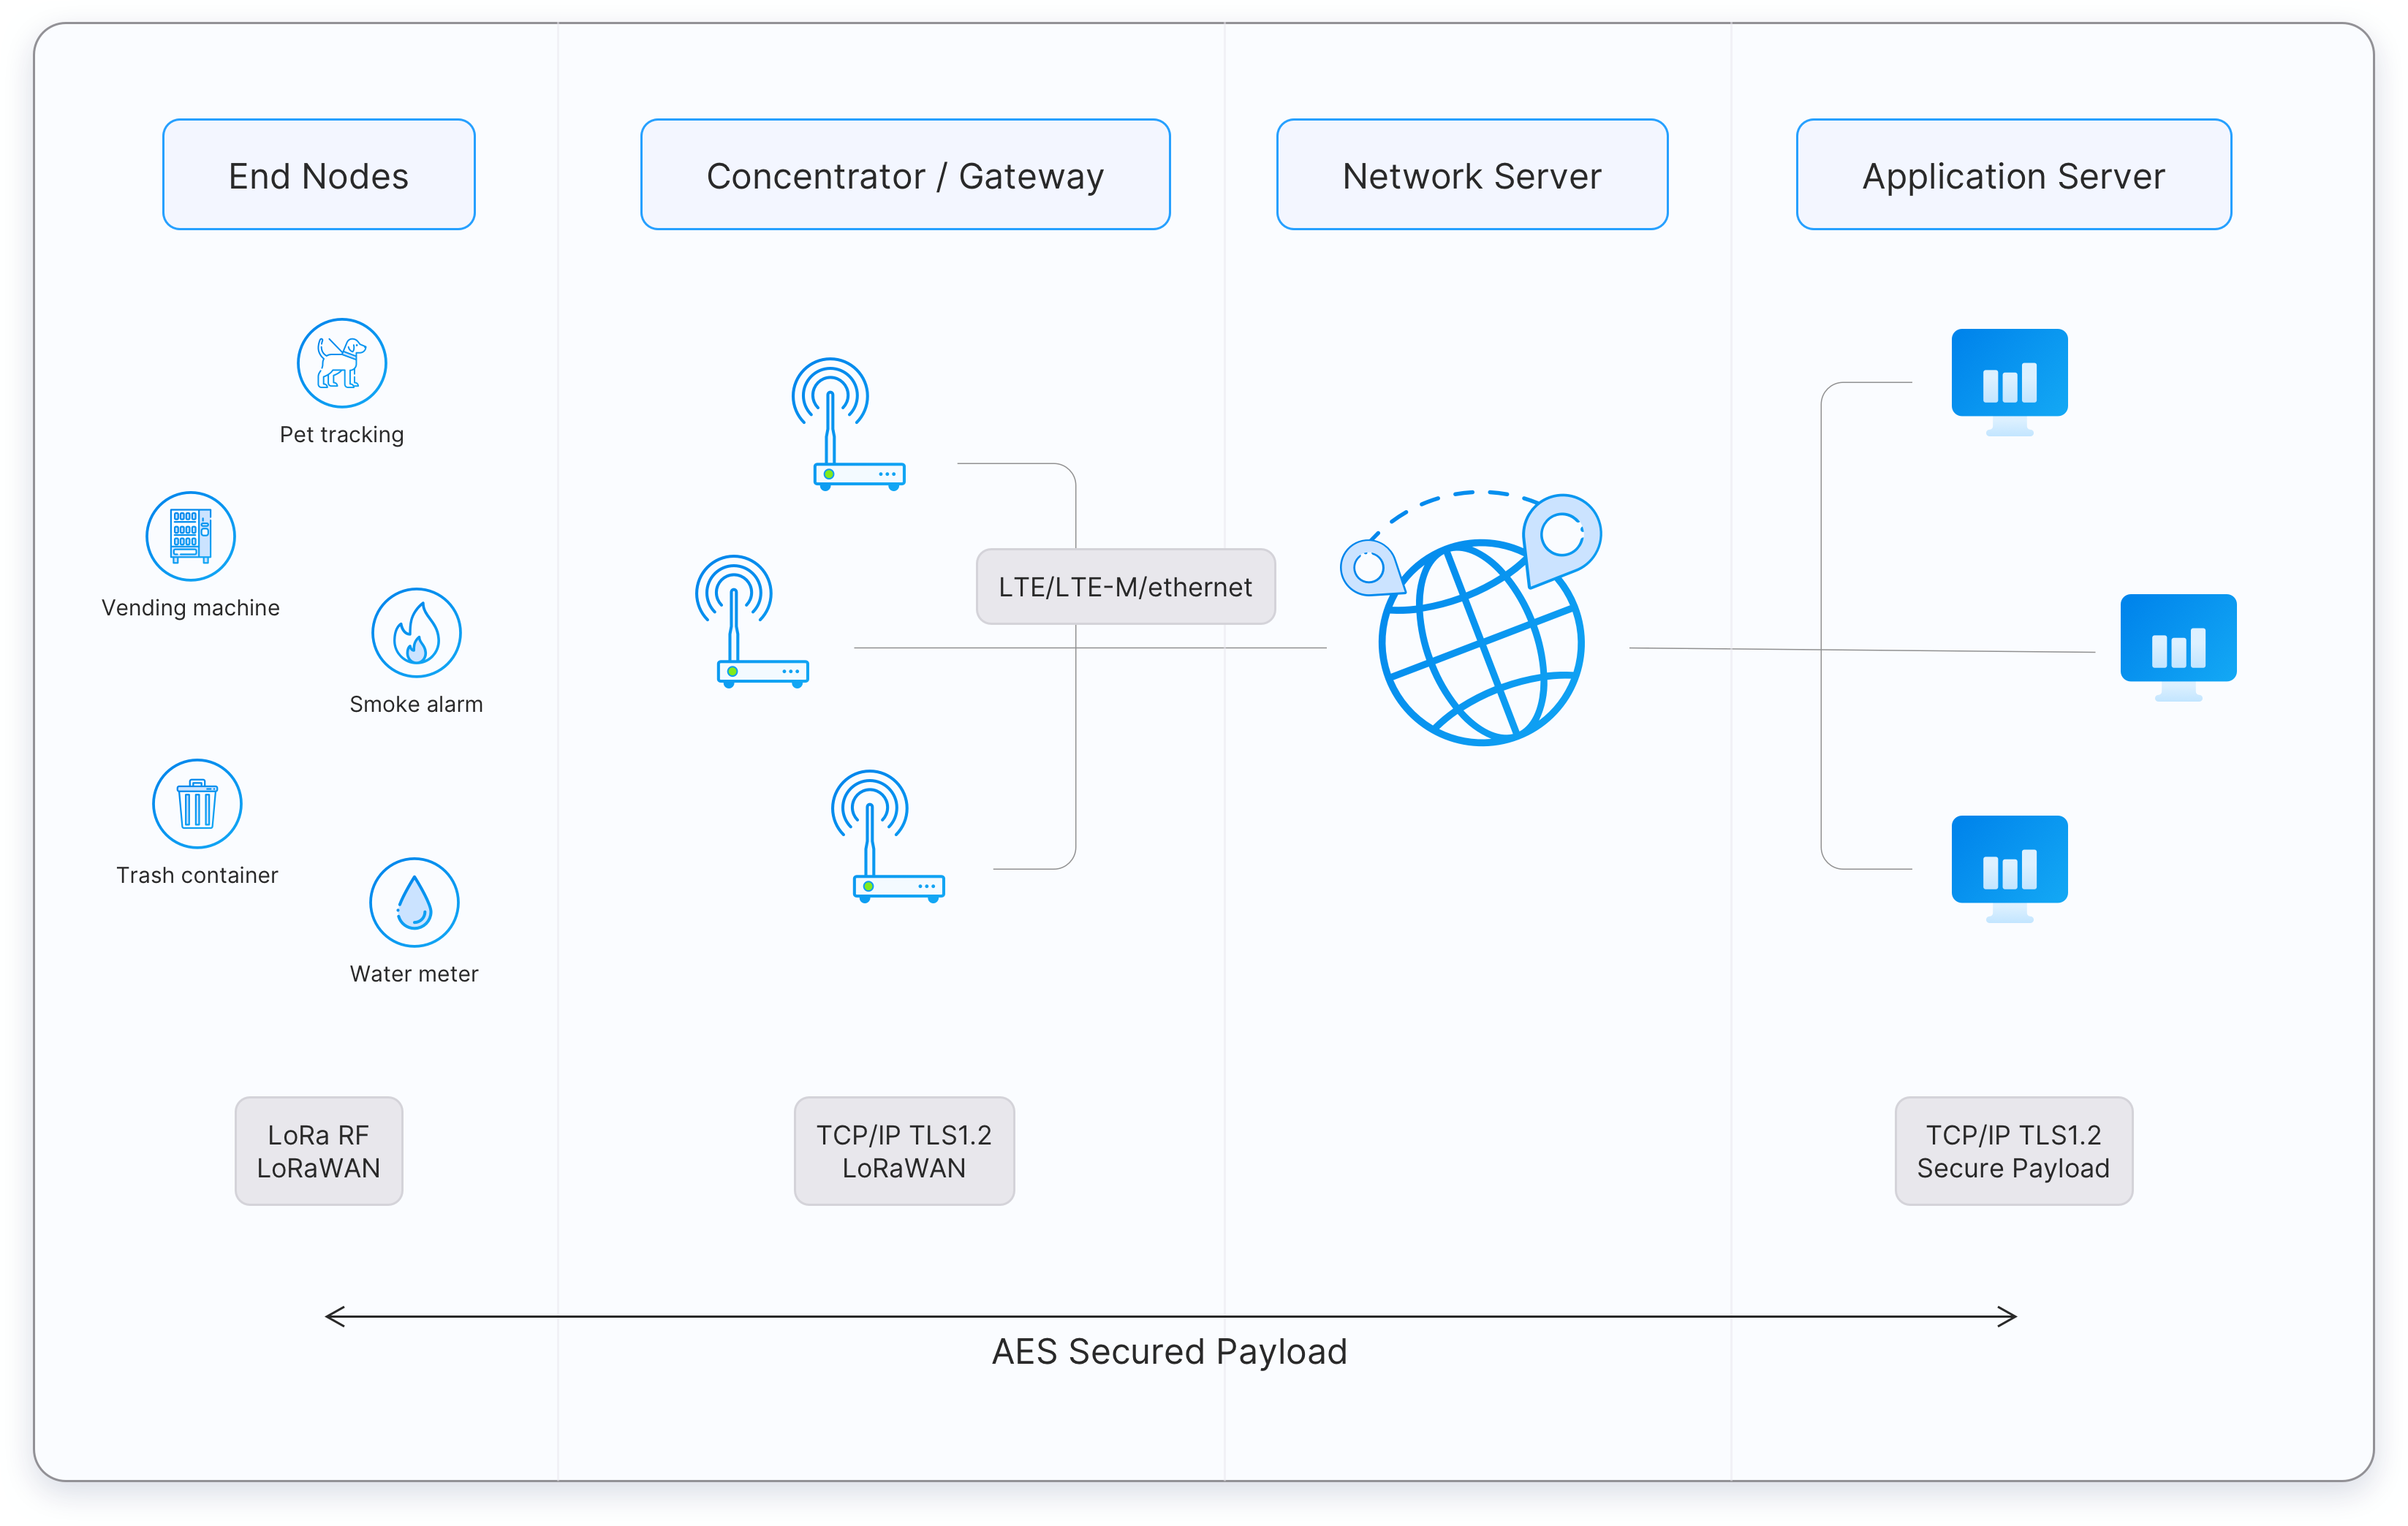
\includegraphics[width=1\textwidth]{pictures/lorawan-structure/lorawan-architecture.png}
    \caption{\ac{LoRaWAN} network structure~\protect\cite{the_things_industries_bv_lorawan_nodate}}\label{pic:lorawan-network-structure}
\end{figure}

The \ac{LoRaWAN} network architecture, as seen in \cref{pic:lorawan-network-structure} consists of four main components~\cite[p. 8]{lora_alliance_inc_lorawan_2017}:

\begin{itemize}
    \item The end nodes (also called devices or motes),
    \item the gateways (also called concentrators or base stations),
    \item the \ac{LNS}, and
    \item the \acp{AS}.
\end{itemize}

\ac{LoRaWAN} data rates typically range from 0.3 kbps to 50 kbps, depending on the region and the \ac{LoRa} modulation used~\cite[p. 8]{lora_alliance_inc_lorawan_2017}.

\subsection{Gateways}

\begin{figure}
    \centering
    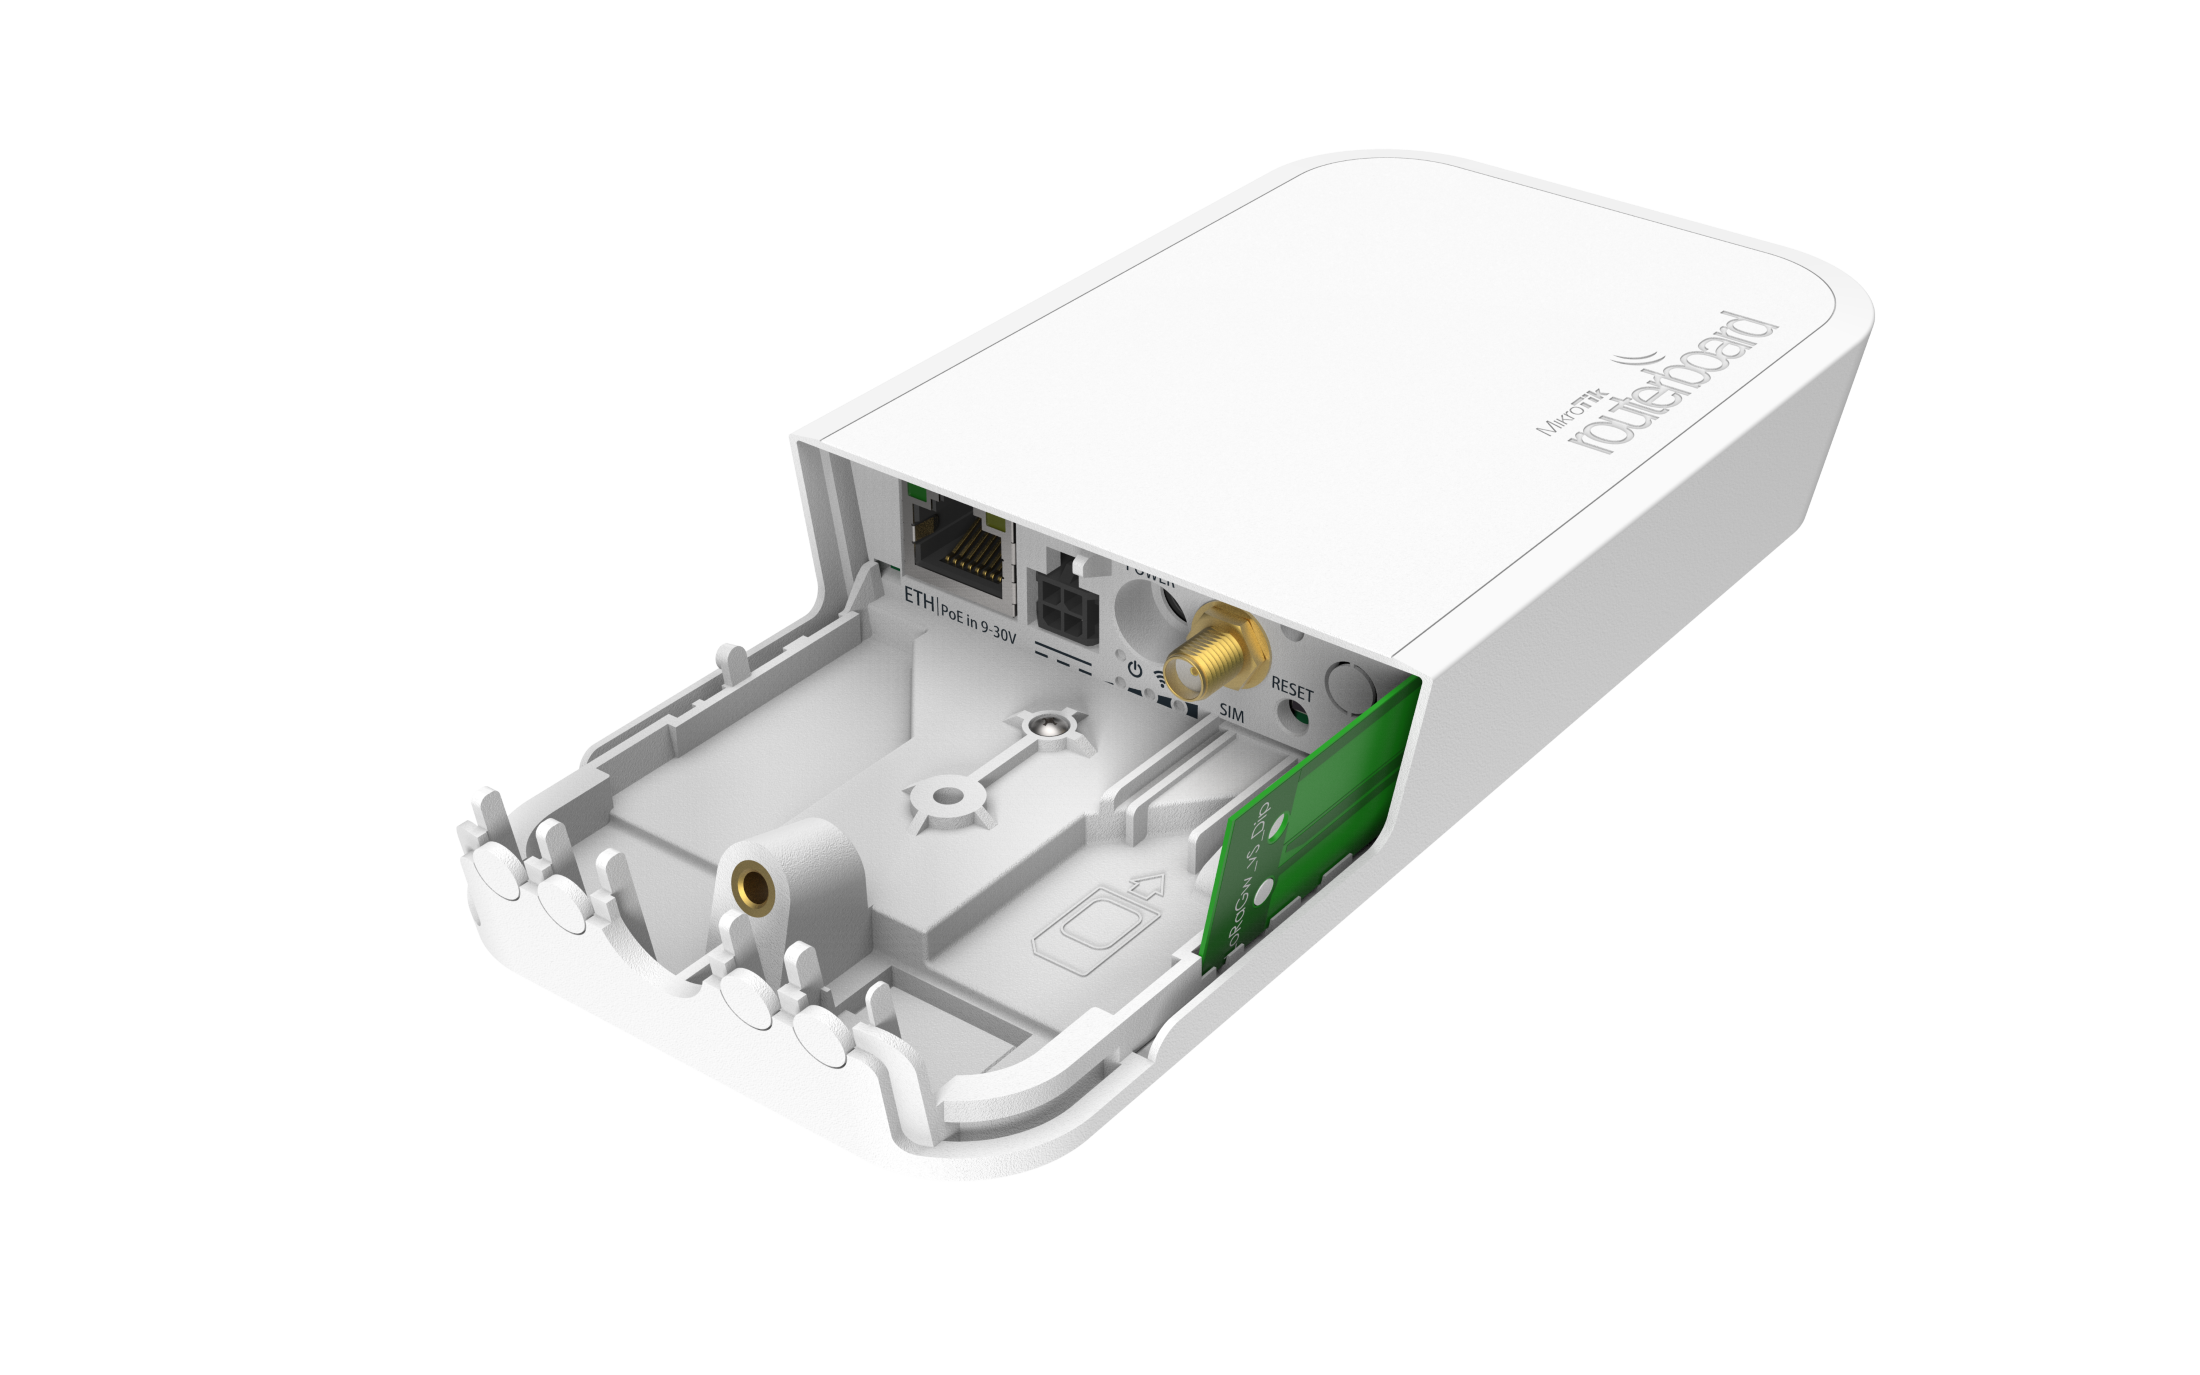
\includegraphics[width=.6\textwidth]{pictures/hardware/gateways/mikrotik-lr8-kit.png}
    \caption{MikroTik wAP LR8 kit Gateway~\protect\cite{the_things_industries_bv_lorawan_nodate}}\label{pic:mikrotik-lr8-kit-gateway}
\end{figure}

A \ac{LoRa} gateway is a device that receives \ac{LoRa} packets (usually from \ac{LoRa} nodes/end devices) and forwards them to the \ac{LoRaWAN} server.

\ac{LoRa} gateways are usually based on a \ac{LoRa} concentrator, which is a \ac{RF} front-end module that receives \ac{LoRa} packets and forwards them to the gateway's \ac{CPU} using a serial interface.
The \ac{CPU} processes the incoming data and forwards the packets to the \ac{LoRaWAN} server.

To achieve the connection to the \ac{LoRaWAN} server, the gateway needs to be connected to the internet.
This connection is also called \emph{backhaul}.
The most widely used methods to realize this are Ethernet/\ac{LAN}, Wi-Fi and \ac{LTE} connections.

One example of a gateway used during this thesis and therein installed in Furtwangen is the \emph{MikroTik wAP LR8 kit}, as seen in \cref{pic:mikrotik-lr8-kit-gateway}.
This gateway is specified as suitable for outdoor usage, making it a good choice for the deployment in Furtwangen on top of (among others) the roof of the student dorm \ac{GHB}.

\begin{figure}
    \centering
    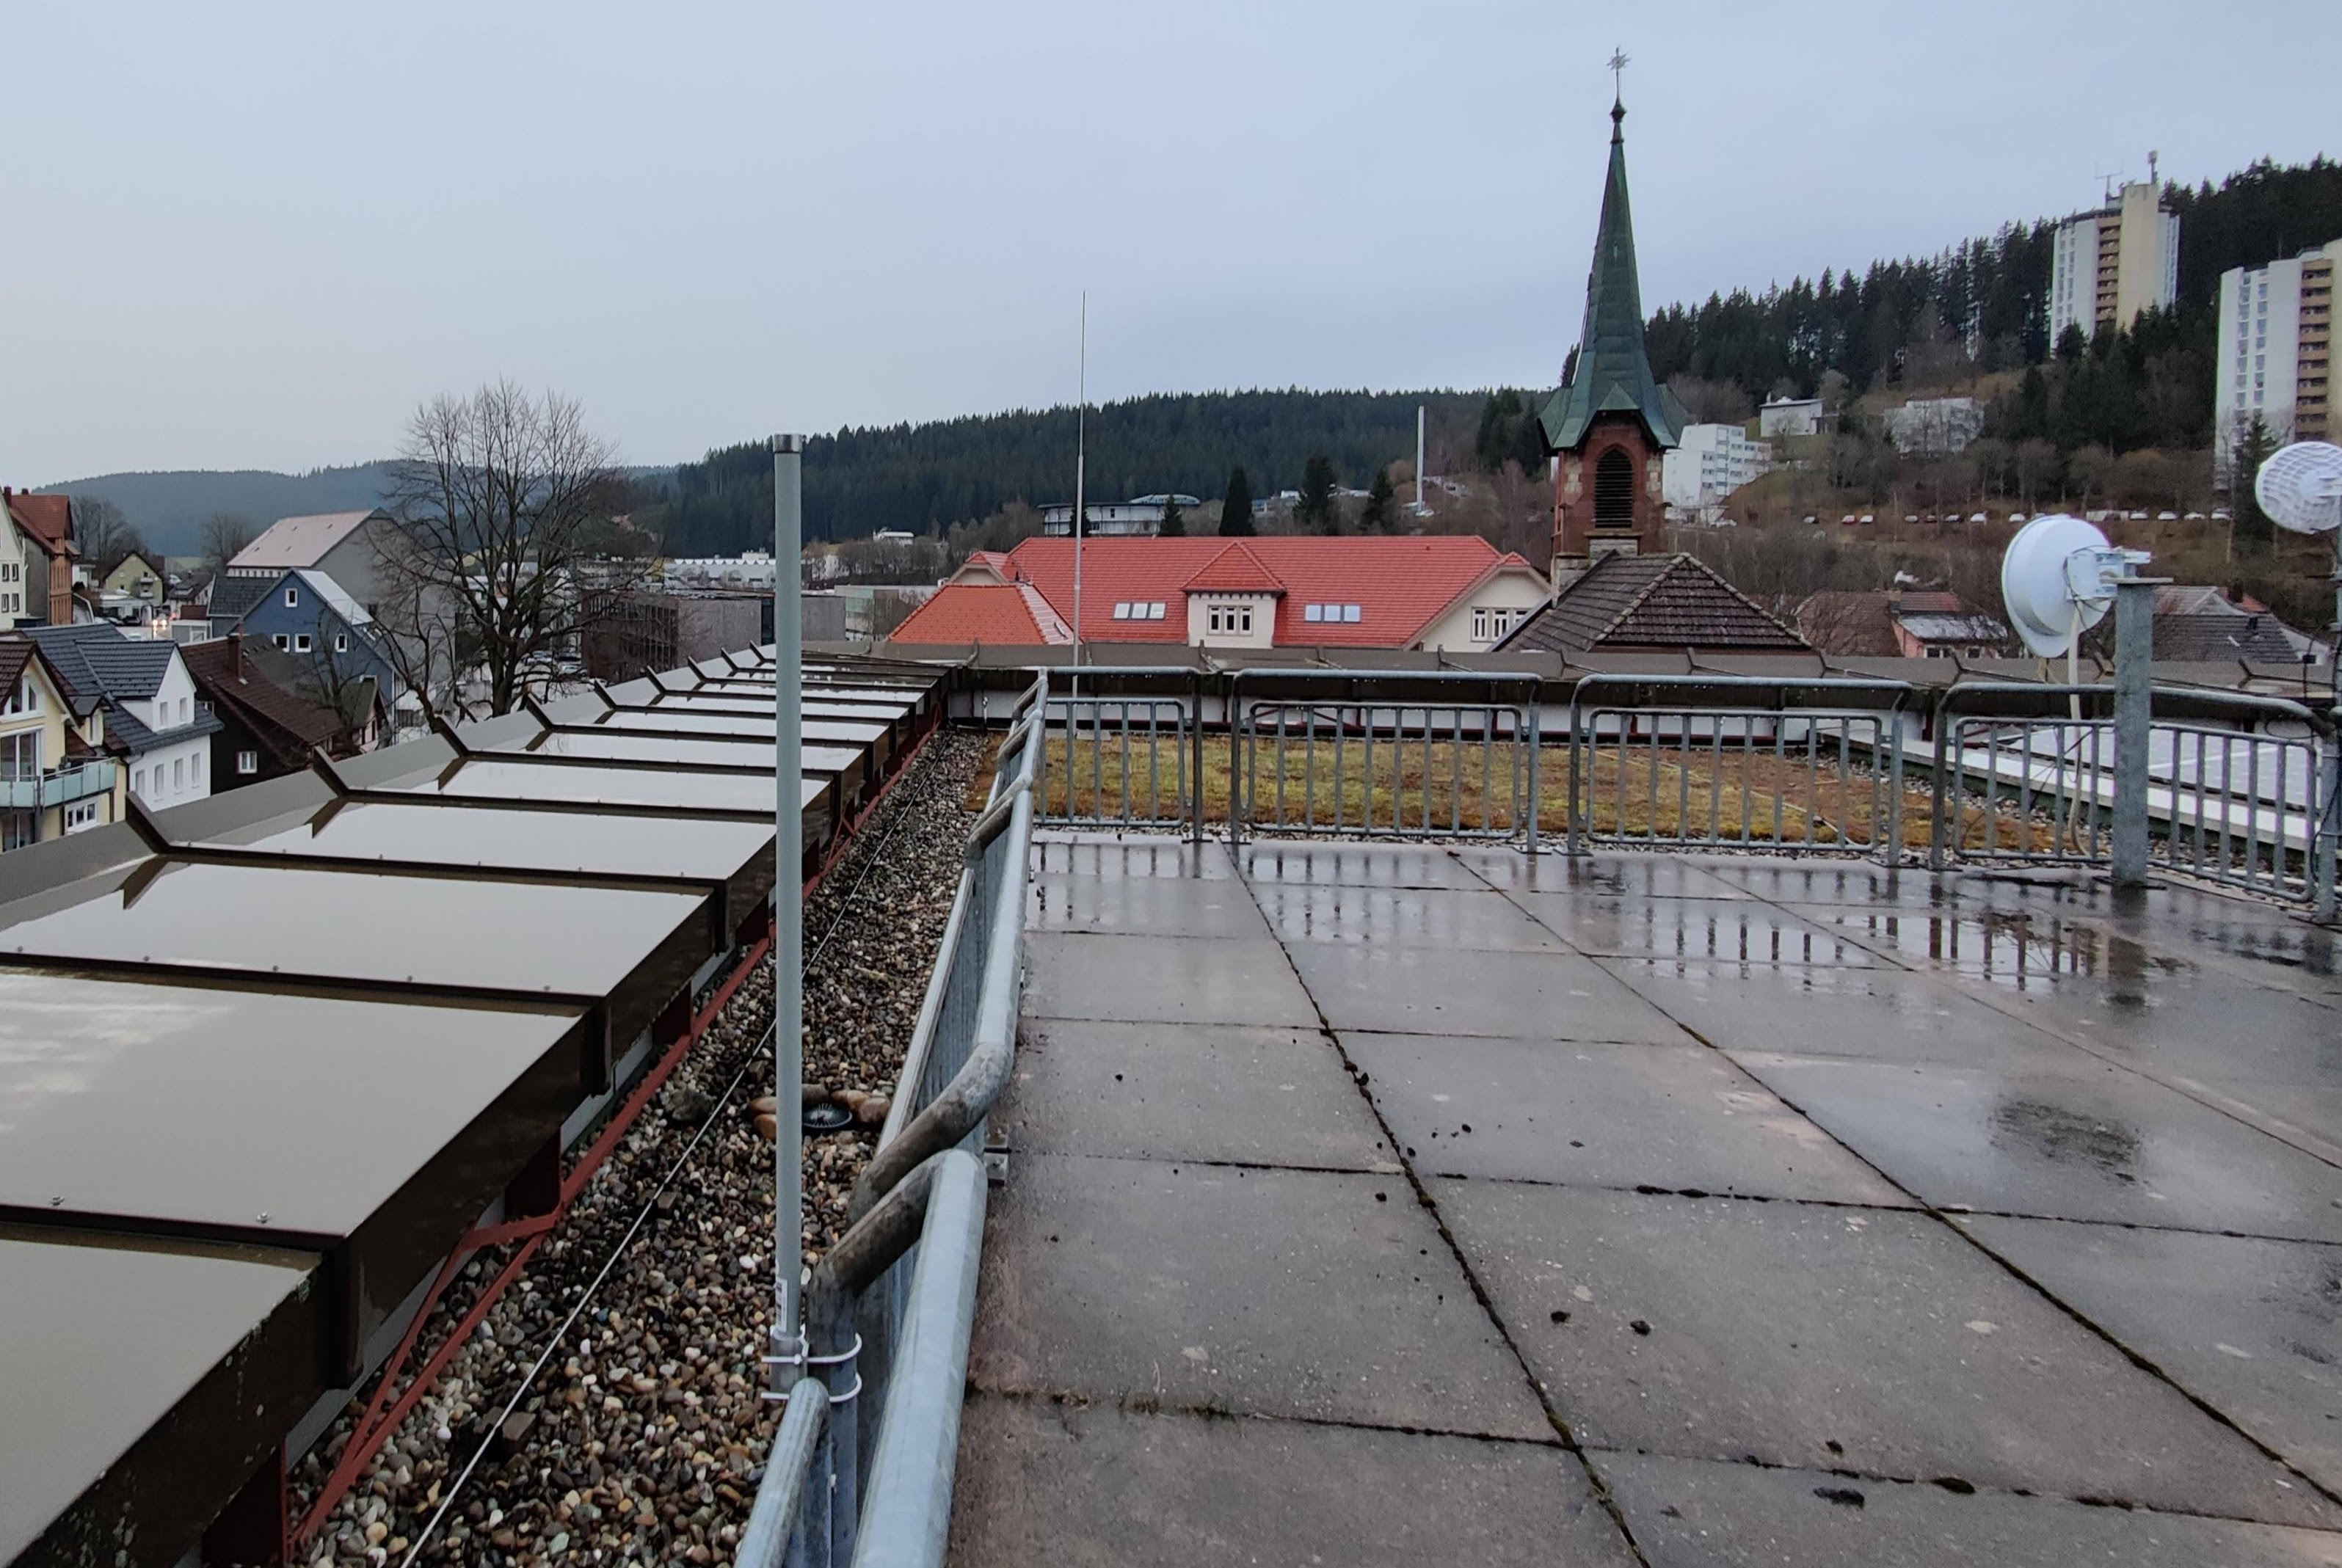
\includegraphics[width=0.6\textwidth]{pictures/hardware/gateway-deployment/mikrotik-antenna-c-building.jpg}
    \caption{The MikroTik antenna installed on top of the \ac{HFU} C building}\label{pic:mikrotik-antenna-c-building}
\end{figure}

While gateways like these usually have a built-in antenna, their range is only sufficient for covering small to medium-sized buildings or areas.
It is, however, also possible to use external antennas if it is necessary to cover a much larger area as was the case in this thesis since a medium to long range localization of \ac{LoRa} nodes was the goal.
While there are many choices for external antennas, as far as the MikroTik gateway is concerned, the choice was made to also use the external \ac{LoRa} antenna supplied by MikroTik, as it is specifically designed for the MikroTik gateway and thus should be a good match.
The deployment of this antenna on top of the \ac{HFU} C building is shown in \cref{pic:mikrotik-antenna-c-building}.

\subsection{Data Transmission}

In LoRaWAN, data transmissions to and from the end nodes are called \emph{uplink} and \emph{downlink}, respectively~\cite[p. 12]{lora_alliance_inc_lorawan_2017}.

Uplinks are relayed to the network server by one or more gateways from the end node.
Downlinks, however, are only sent from the network server to the end node using a single gateway.
\subsection{Device Classes}

\ac{LoRaWAN} defines three classes of devices that offer different variations of the trade-off between power consumption and data rate/availability~\cite[p. 10]{lora_alliance_inc_lorawan_2017}.

\subsubsection{Class A}

\begin{figure}
    \centering
    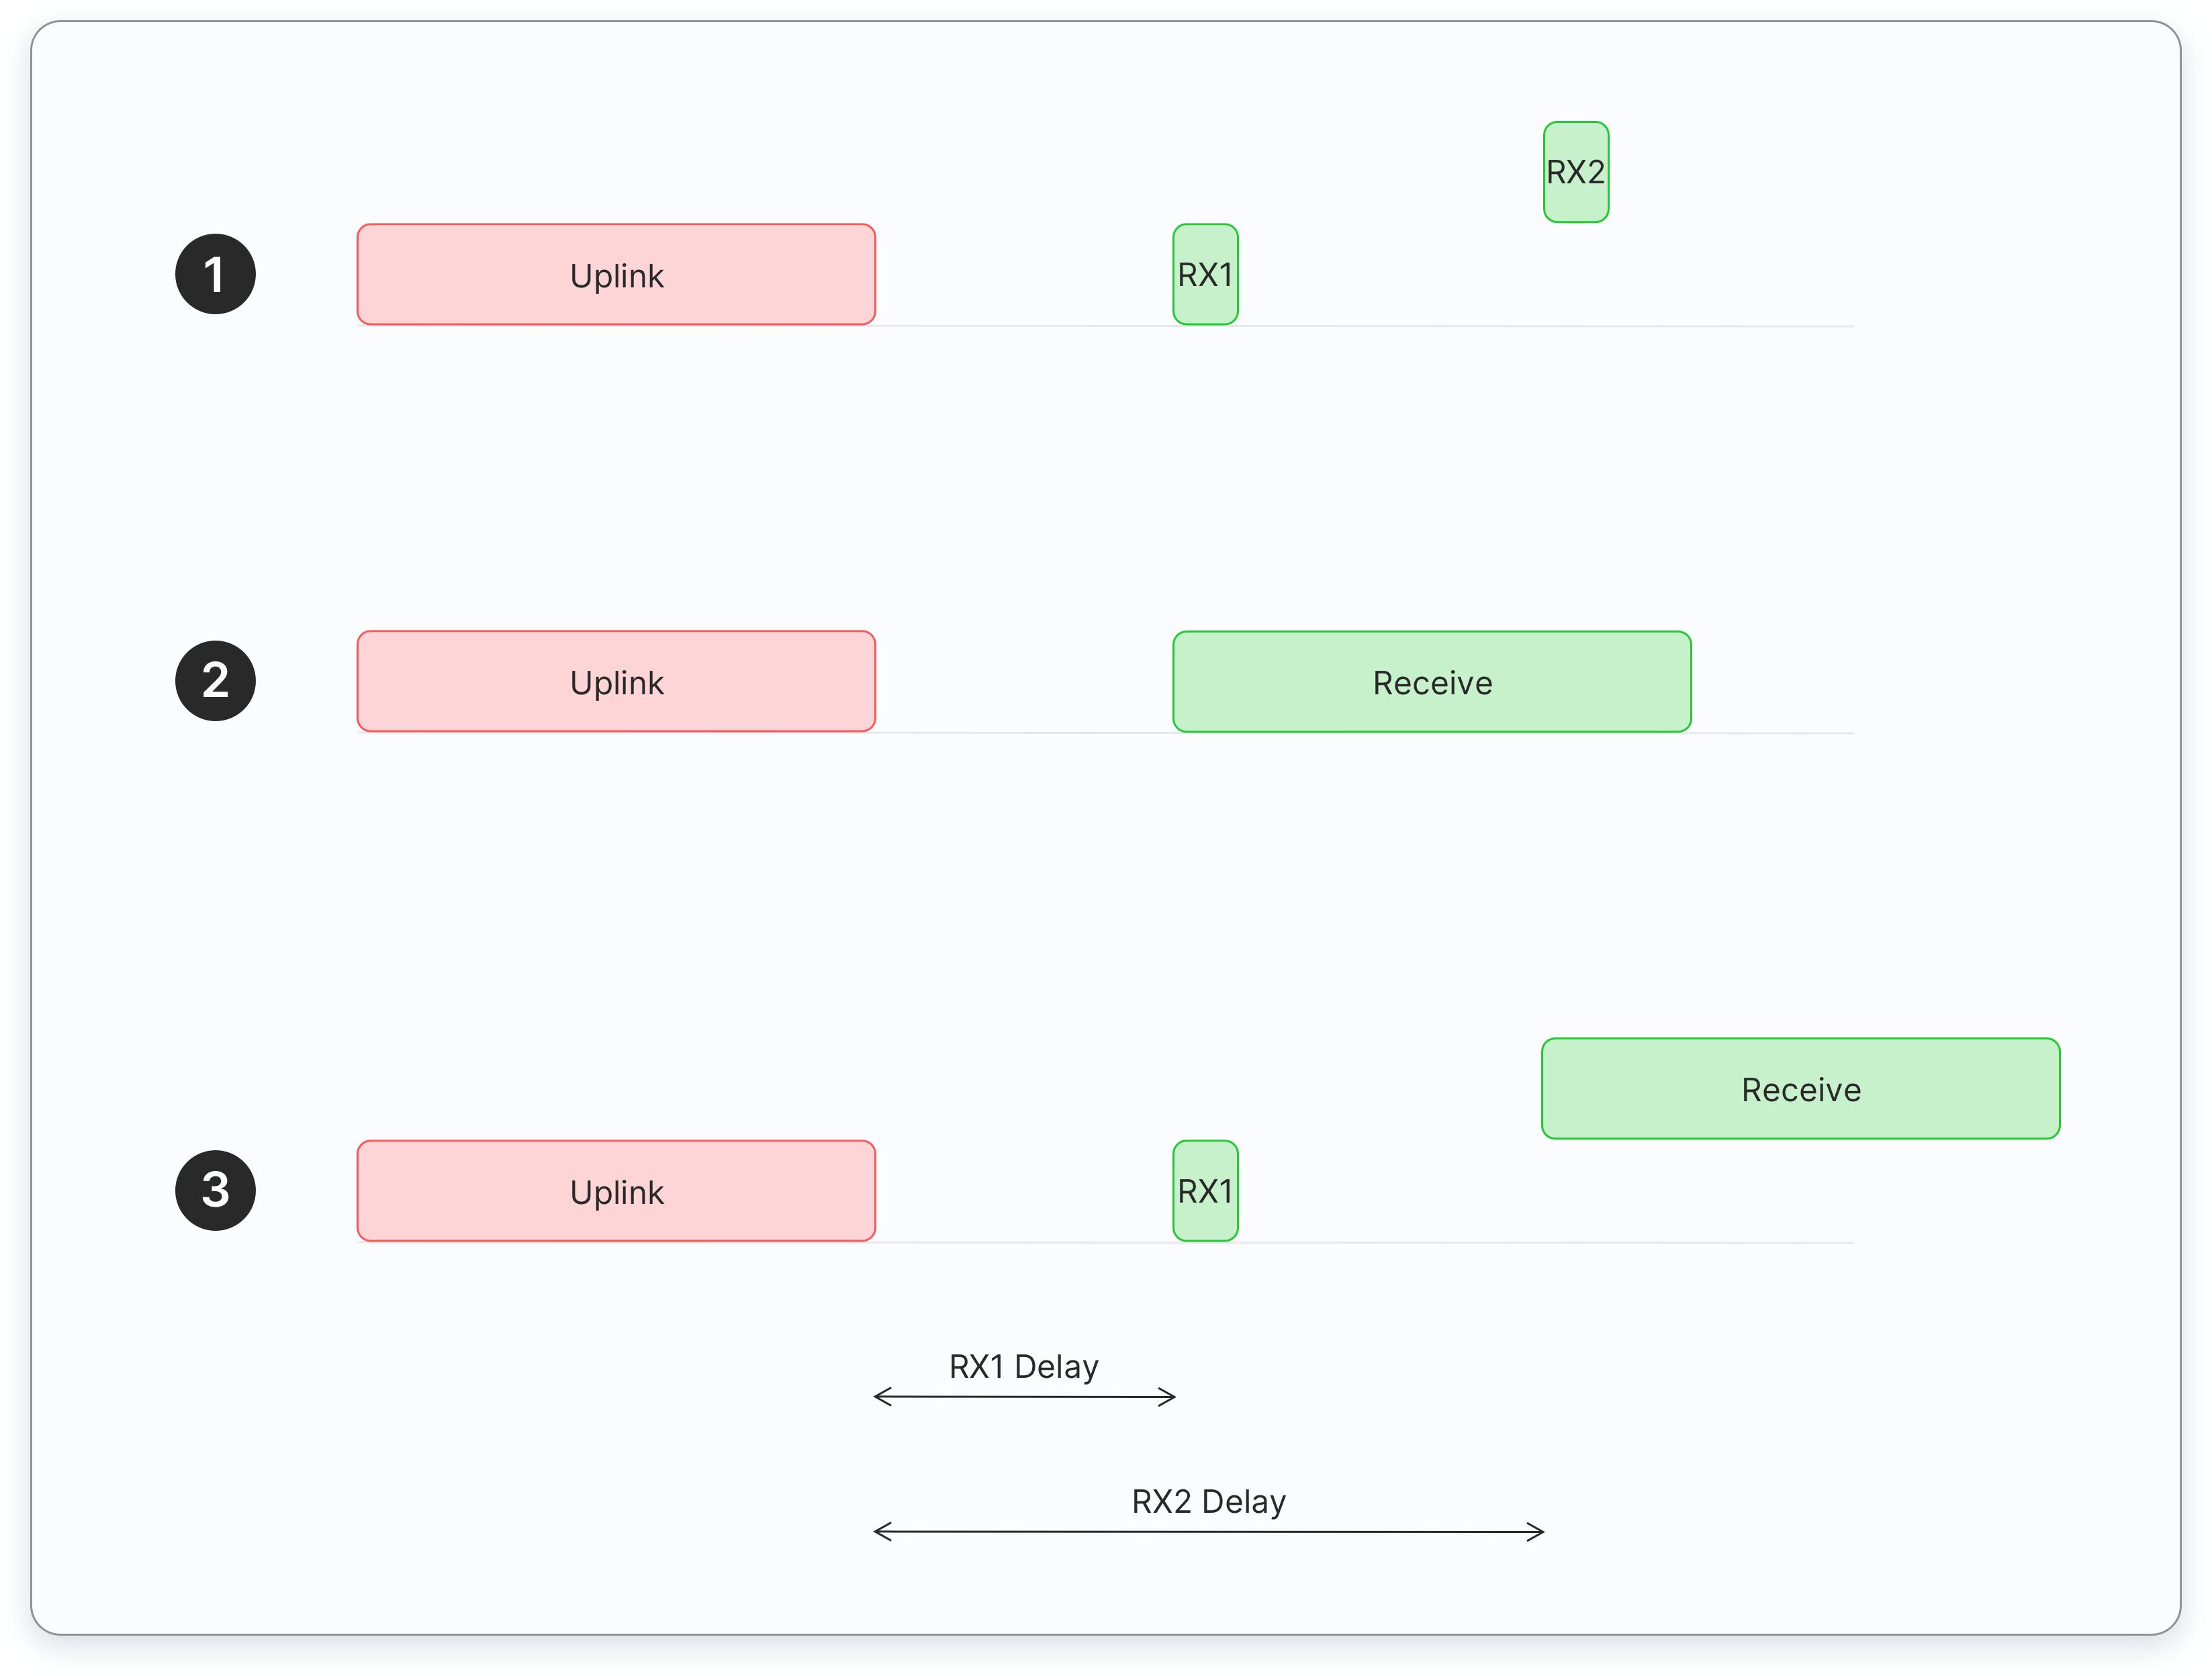
\includegraphics[width=1\textwidth]{pictures/device-classes/class-a.png}
    \caption{\ac{LoRaWAN} Device class A communication schema~\protect\cite{the_things_industries_bv_device_nodate}}\label{pic:lorawan-device-class-a-schema}
\end{figure}

Class A is used for devices that need to consume as little power as possible.
Every \ac{LoRaWAN} device must support the Class A mode~\cite[p. 11]{lora_alliance_inc_lorawan_2017}.
A communication in Class A is always initiated by the end device itself.

Bidirectional communication is possible in Class A through the use of two downlink receive windows during which it is possible for the \ac{LNS} to send data to the device.
This can be seen in \cref{pic:lorawan-device-class-a-schema}.
This also makes it impossible for the \ac{LNS} to send data to the device at any other time.

Class A consumes the least amount of power of the three classes, since the devices itself may specify when and how often they want to communicate with the \ac{LNS}.

\subsubsection{Class B}

\begin{figure}
    \centering
    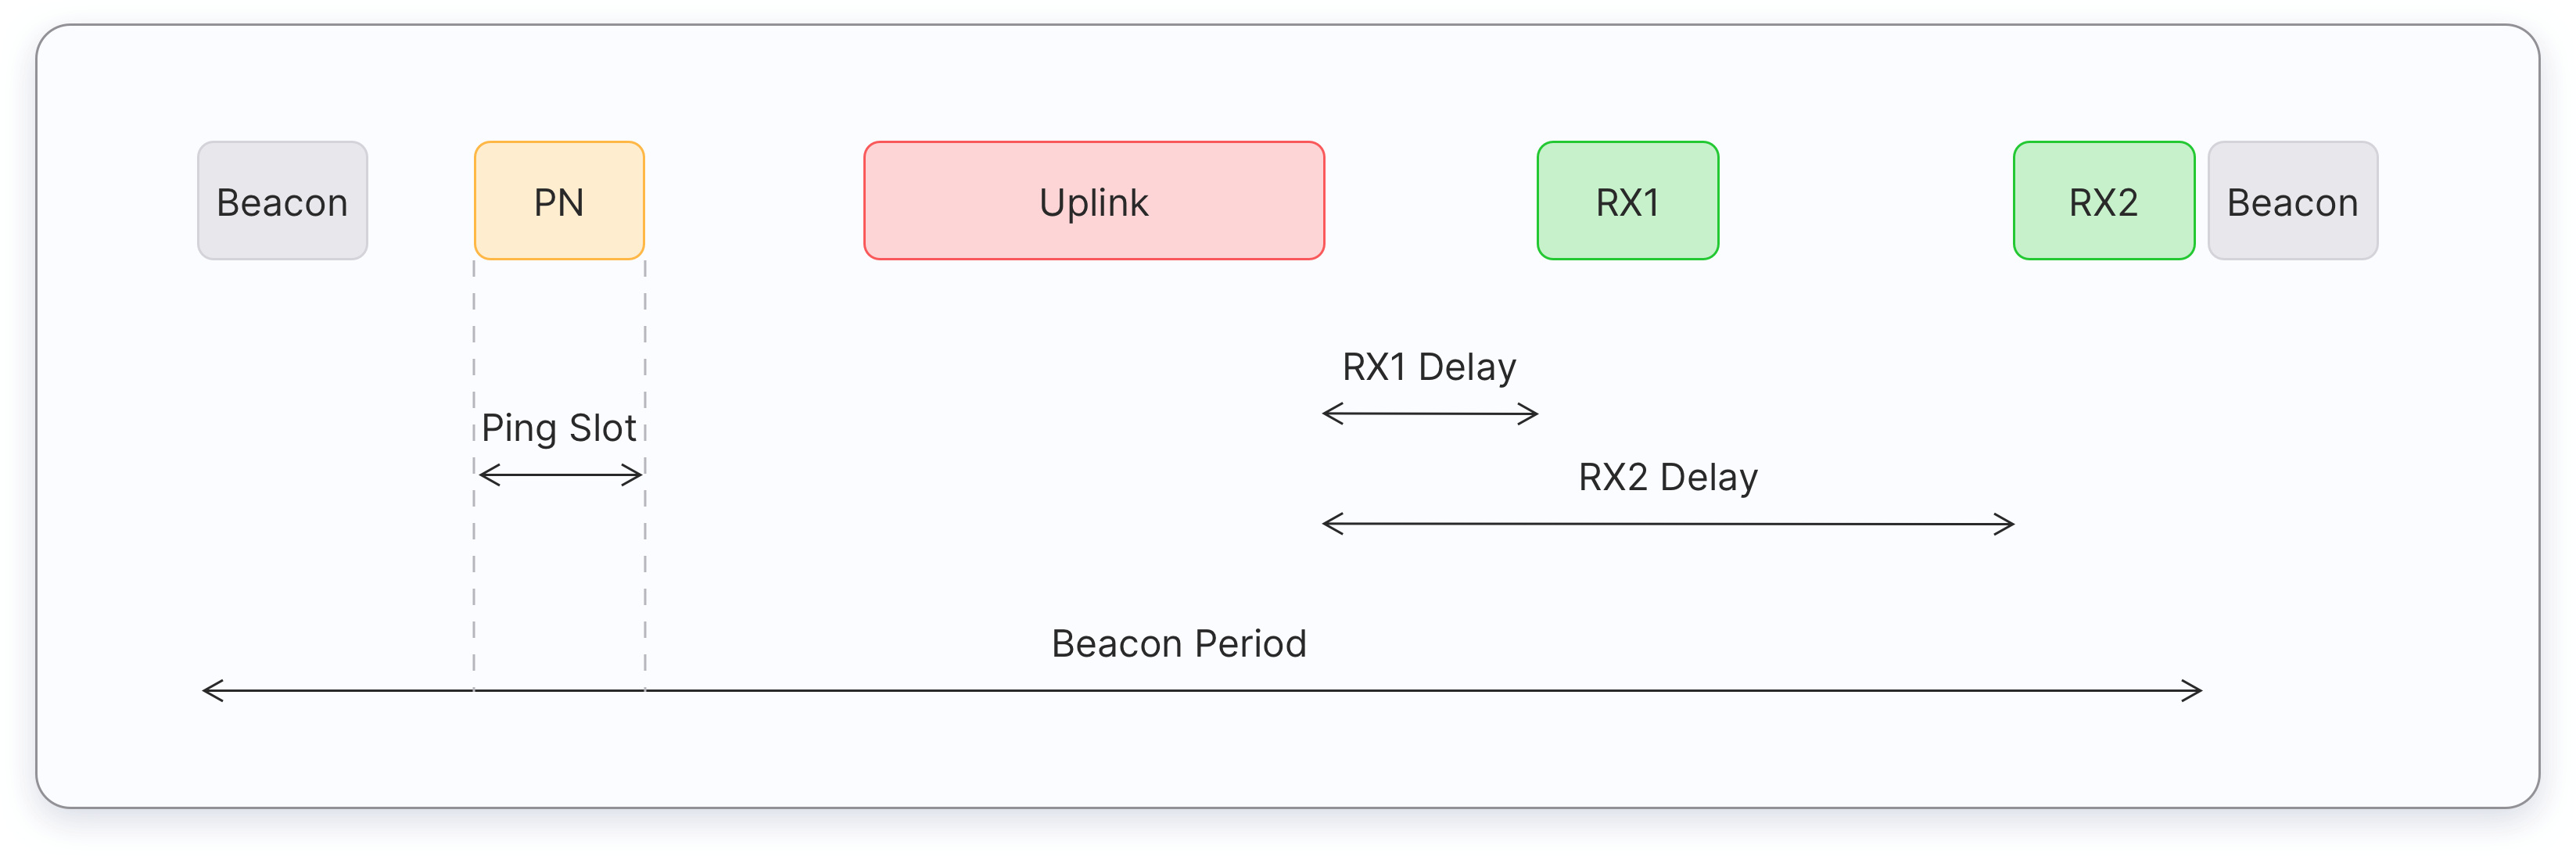
\includegraphics[width=1\textwidth]{pictures/device-classes/class-b.png}
    \caption{\ac{LoRaWAN} Device class B communication schema~\protect\cite{the_things_industries_bv_device_nodate}}\label{pic:lorawan-device-class-b-schema}
\end{figure}

In addition to class A, class B devices are also able to receive downlink messages from the \ac{LNS} during dedicated downlink receive windows.
In order to realize this without the need for a per-device \ac{RTC}, class B devices receive time synchronized beacons from the gateways.
The communication schema for class B devices can be seen in \cref{pic:lorawan-device-class-b-schema}.

These scheduled downlink windows result in a higher power consumption for class B devices, since those need to be awake during these windows.

\subsubsection{Class C}

\begin{figure}
    \centering
    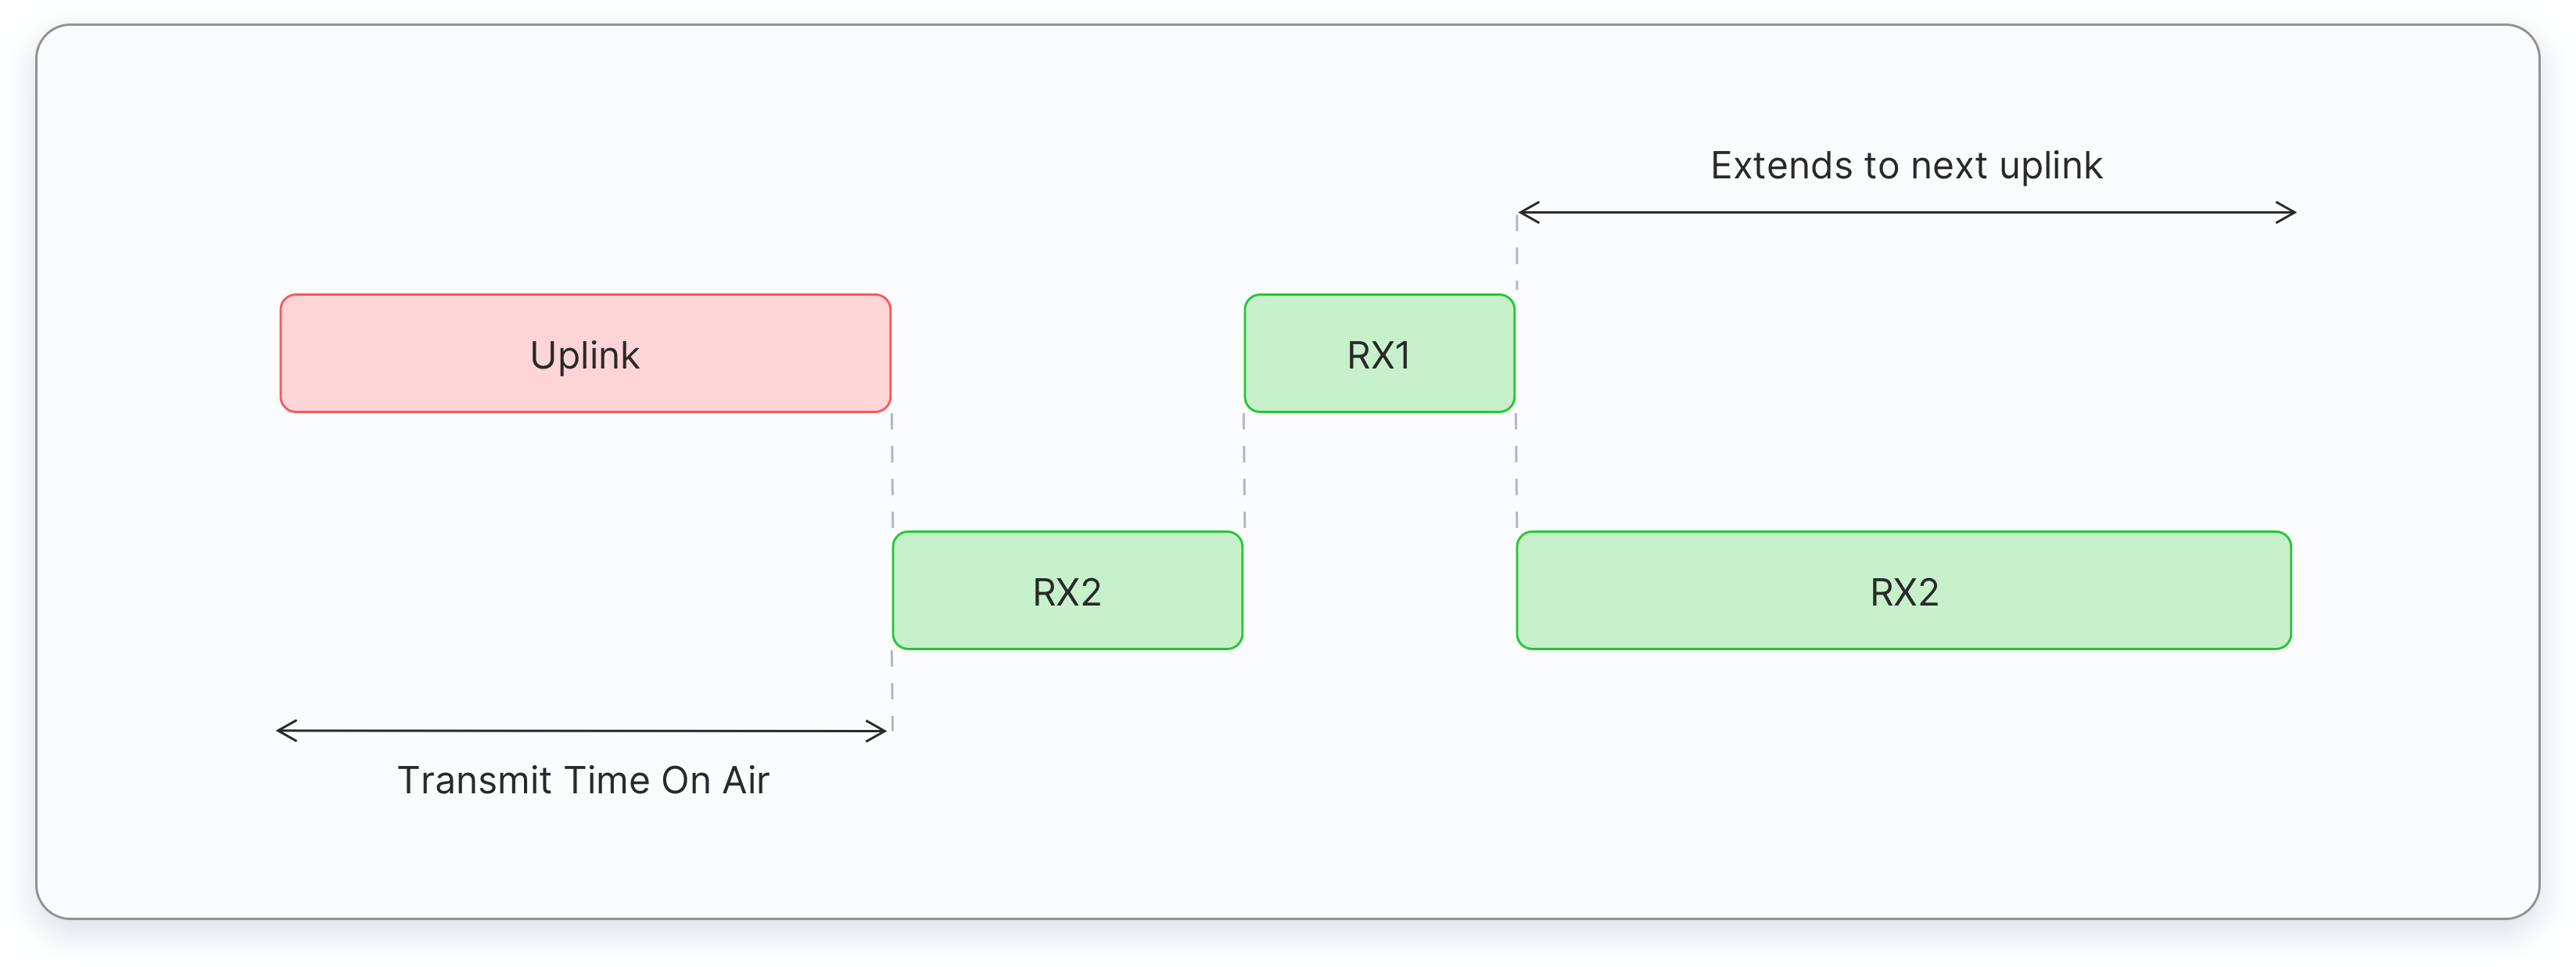
\includegraphics[width=1\textwidth]{pictures/device-classes/class-c.png}
    \caption{\ac{LoRaWAN} Device class C communication schema~\protect\cite{the_things_industries_bv_device_nodate}}\label{pic:lorawan-device-class-c-schema}
\end{figure}

Class C devices, when not currently transmitting an uplink message, are always listening for downlink messages from the \ac{LNS}.
In essence, they keep the downlink windows as specified in class B open all the time as seen in \cref{pic:lorawan-device-class-c-schema}.

Devices in class C consume the most power, since they are always listening for downlink messages.
The fact that they are always reachable by the \ac{LNS} also makes them the most suitable for applications that require a high data rate or a reliable accessibility via downlink.

\subsubsection{Conclusion}

As far as this thesis was concerned, only devices with class A were used.
This is because class B and C use significantly more power than class A because they keep their radio on for extended periods of time, which is a problem for battery-powered devices.

In their work ``Comparison of LoRaWAN Classes and their Power Consumption'', Cheong et al.\ show that a device in Class C  would need a battery around 19 times as large as a Class A device to achieve the same battery life with a packet size of 115 bytes and a transmission interval of 1 hour~\cite{cheong_comparison_2017-1}.
As mobile devices that have the need to be located are usually battery-powered, class A is the most viable option for them.

\section{\acf{TTN}}

\begin{figure}
    \centering
    
\includegraphics[width=0.3\textwidth]{pictures/logos/TTN-logo.eps}
    \caption{\acf{TTN} logo~\protect\cite{the_things_industries_bv_quick_nodate}}
\end{figure}

\ac{TTN} provides a free to use \ac{LNS} that supports a global community of people building \ac{LoRaWAN} applications.

While, officially, it is called \emph{The Things Stack Community Edition} since 2021, it is still commonly referred to as \acf{TTN}~\cite{the_things_industries_bv_what_2022}.
Its users provide \ac{TTN} with gateways that other users can use, making it a decentralized and crowdsourced \ac{LoRaWAN} network.

\subsection{Gateways}

Gateways can forward \ac{LoRaWAN} packets that it receives to the \ac{LNS} in two major ways:

\subsubsection{\acf{SUPF}}

The \acl{SUPF} is a piece of software used to connect \ac{LoRa} gateways to the \ac{LNS}~\cite{the_things_industries_bv_semtech_2022}.
The \ac{SUPF} relays \ac{LoRaWAN} packets that it receives from its connected \ac{LoRa} concentrator to the \ac{LNS} using the \ac{UDP} protocol.

It may be configured using JSON files such as \lstinline{global_conf.json} and \lstinline{local_conf.json}.

\ac{TTN} marked the \acl{SUPF} as deprecated, since it ``has many security and scalability drawbacks``~\cite{the_things_industries_bv_semtech_2022}.
It is advised to use the \acl{LBS} protocol instead.

\subsubsection{\acf{LBS}}

\begin{figure}
    \centering
    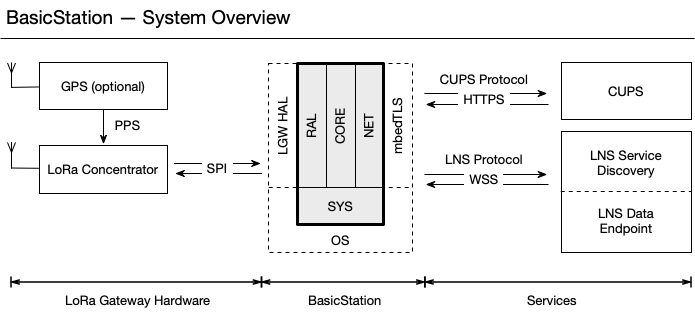
\includegraphics[width=0.9\textwidth]{pictures/lorawan-structure/lora-basics-station-structure.png}
    \caption{\acf{LBS} communication schema~\protect\cite{semtech_lora_developer_portal_lora_2022}}\label{pic:lora-basics-station-schema}
\end{figure}

Since \ac{TTN} v3, using the \ac{TCP}-based \acl{LBS} protocol is recommended over the \ac{SUPF} to connect gateways to the \ac{LNS}~\cite{the_things_industries_bv_semtech_2022}.

\ac{LBS} uses \ac{TLS}-encrypted \ac{TCP} connections with token-based authentication to relay \ac{LoRaWAN} packets to the \ac{LNS}~\cite{the_things_industries_bv_lora_2022}.

The two main components of \acl{LBS} are the \ac{LNS} itself as well as the \acf{CUPS}.
The communication schema can be seen in \cref{pic:lora-basics-station-schema}.

The \ac{LNS} is responsible for handling the \ac{LoRaWAN} packets whereas the \acl{CUPS} is responsible for handling the configuration of the gateways.

While \ac{CUPS} is not strictly necessary for sending actual \ac{LoRaWAN} packets, it simplifies the management of gateways and their configuration.
When a gateway is configured with \ac{CUPS}, it will automatically receive its configuration from the \ac{LNS} and be authenticated to work with it~\cite{the_things_industries_bv_lora_2022}.

\section{\acf{TTNM}}

\acf{TTNM} was created by engineer JP Meijers in 2015~\cite{linkedin_23_nodate}.
He first created it as a personal project to map the range of his own \ac{LoRaWAN} gateway.
However, the project has since been expanded to map the coverages of almost all gateways registered in the public \ac{TTN} network~\cite{the_things_network_jp_2018}.

\subsection{Data collection}

\acl{TTNM} works by using \ac{LoRaWAN} nodes with \ac{GPS} modules that send their location to the \ac{TTN} network via uplink messages.
Alongside the location information, those nodes' messages that are processed by \ac{TTN} also include information about which gateways received them.

Hence, \acl{TTNM} can use the information about which gateways received the message and the location information of the nodes' \ac{GPS} modules.
This is done by means of a \emph{webhook} that sends the data to an endpoint of the \acl{TTNM} \ac{API} whenever a node sends a message to the \ac{TTN} network.
With this data, it can build a map displaying the coverage of \ac{LoRaWAN} gateways in the \ac{TTN} network.

\subsection{Frontend data views}

\begin{figure}
    \centering
    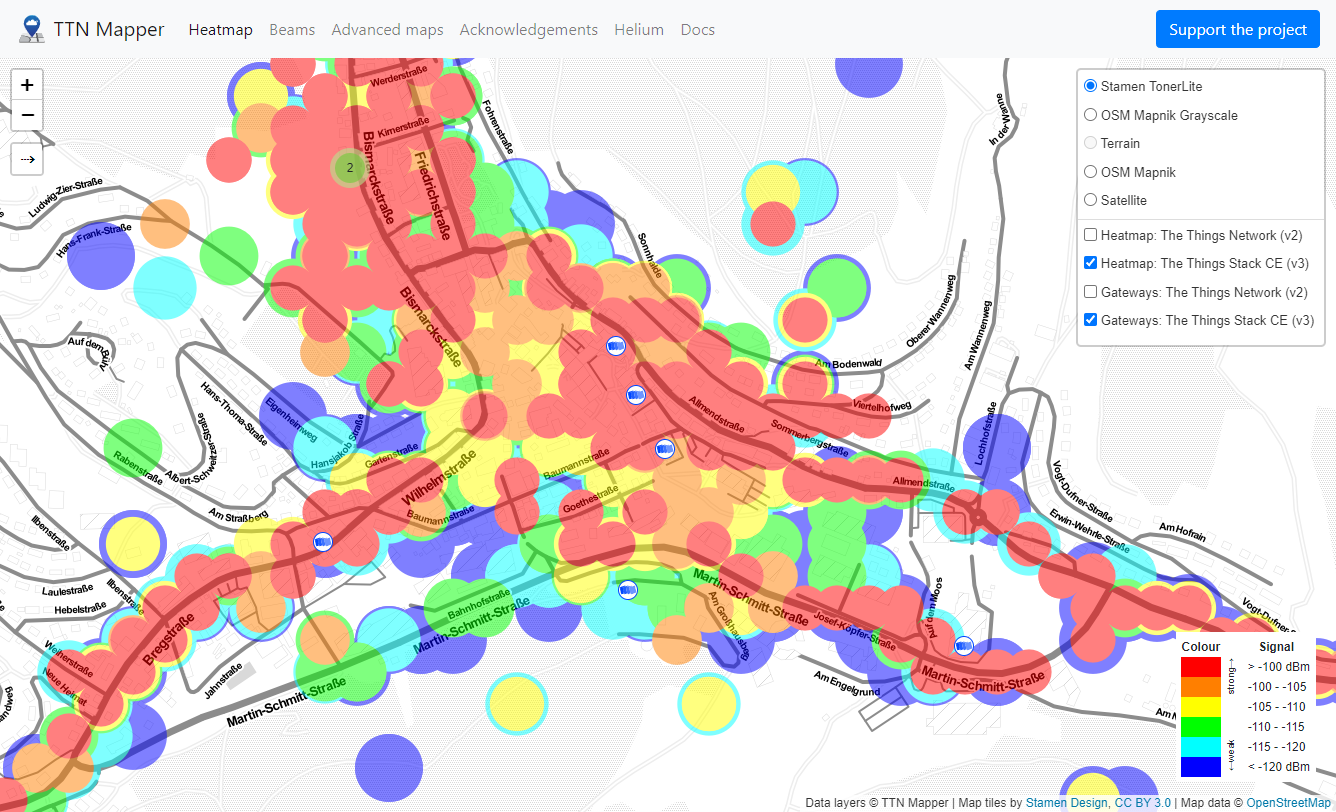
\includegraphics[width=1\textwidth]{pictures/ttn-mapper/heatmap_with_gateways.png}
    \caption{Screenshot of \ac{TTNM}'s \emph{heatmap} view with some gateways visible (small blue and white circles) in the Furtwangen area~\protect\cite{ttn_mapper_ttn_2023}}\label{pic:ttn-mapper-heatmap-with-gateways}
\end{figure}

\Cref{pic:ttn-mapper-heatmap-with-gateways} shows a screenshot of \acl{TTNM}'s heatmap view.
This page displays an interactive world map with a heatmap overlay.
It shows the coverage of \ac{LoRaWAN} gateways in the \ac{TTN} network by using and aggregating data that has been collected over the lifetime of the service.
Additionally, any gateway that has received at least one message from a \ac{GPS}-enabled \ac{LoRaWAN} node and has its location accessible from \ac{TTN} is displayed on the map.

\subsection{Data access}

As far as this thesis is concerned, \acl{TTNM} provides a way to access \ac{RSSI} and location data points for measurements done by \ac{GPS}-enabled \ac{LoRaWAN} nodes.

% Mention open API endpoints for accessing data with .csv files
\ac{TTNM} provides a (partly) open \ac{REST} \ac{API} that can be used to access the data that has been collected by it.
Data can be requested based on the end device that sent the message or the gateway that received it.
Additionally, the data can be filtered by the time that it was recorded on.
The data is provided in graphical (map-based) form as well as in \ac{CSV} files.
There is an additional non-documented part of the \ac{API} that can be used to access the data in \ac{JSON} form.
This was the part of the \ac{API} that was used most for this thesis.

\subsection{Importance for this thesis}\label{sec:ttn-mapper-importance}

The data that is provided via the \ac{TTNM} \ac{REST} \ac{API} was the core of this thesis.
The \ac{TTNL} application that will be described in \cref{section:ttnl} was created to access this \ac{API} and request its data to make it possible to perform advanced queries on it.
Such queries were not possible with the \ac{TTNM} \ac{API} alone, as it doesn't provide direct access to its underlying \ac{DB} or provide specific endpoints for the data filtering that was needed for this thesis.

Through building a database of \ac{RSSI} and location values, \ac{TTNM} also enables the use of the fingerprinting localization technique, as will be explained in \cref{sec:rssi-fingerprinting}.
This was one of the techniques used to locate devices in this thesis.

\section{Multilateration}\label{sec:multilateration-basics}

In everyday language, people often use the term \emph{triangulation} or when talking about the process of determining the location of a device based on the distance to multiple other devices.
However, triangulation uses the angles between the end device and three reference points to determine the location of the device, hence its name~\cite{yaro_multiangulation_2017}.
This process requires the end device to be able to determine the angles to the reference points, which is needs specific hardware.

The correct term to use when using distances between an end device and multiple receivers to achieve a localization of the end device is \emph{multilateration}.
A specific case of multilateration is \emph{trilateration}, which specifies three receivers to get the ranges from~\cite{ruiz_efficient_2013}.

\section{\acf{GNSS}}

\ac{GNSS} is a generic term for systems that use satellites orbiting the earth to determine the location of a device.
In everyday language, the term \ac{GPS} is often used as a synonym for \ac{GNSS}.
However, \ac{GPS} is only one of the several \ac{GNSS} systems that are currently in use.
\ac{GNSS} system use multilateration to determine the location of end devices as explained in \cref{sec:multilateration-basics}.
To determine the distance from the end device to the satellites, the time it takes for a signal to travel from the satellite to the end device is measured.
This approach is called \acf{ToA}.

\subsection{\acf{GPS}}

\ac{GPS}, in fact, is the \ac{GNSS} system that is operated by the United States of America and is correctly called \emph{NAVSTAR \ac{GPS}}~\cite{department_of_defense_usa_gps_2020}.
The version of GPS the public has access to is called \acf{SPS}.
Additionally, there is the \acf{PPS} that is only available to the military and other authorized users~\cite{department_of_defense_usa_gps_2007}.

Using an iPhone 6, Merry and Bettinger measured the accuracy of \ac{GPS} to be between 7 and 13 meters in an urban environment~\cite{merry_smartphone_2019}.

\subsection{Other \acs{GNSS} systems}

There are several other \ac{GNSS} systems in use or in development by different countries.
For example, the Russian \acf{GLONASS} system, the European \acf{Galileo} system, the Chinese \acf{BDS} system, and the Indian \acf{IRNSS} system.

Most modern user devices such as smartphones support multiple \ac{GNSS} systems to improve the accuracy of the location determination.
For example, one of Samsung's most recent devices as of writing this thesis, the Galaxy S23 Ultra, supports \ac{GPS}, \ac{GLONASS}, \ac{Galileo}, and \ac{BDS}~\cite{gsmarena_samsung_2023}.

The \ac{LoRaWAN} nodes used in this thesis, as described in \cref{subsec:used-lora-nodes}, only use \ac{GPS} to determine their location.

\subsection{\acf{HDOP}}

% Explain HDOP and relevance to GPS accuracy

\section{Localization of devices}


\section{Localization techniques for usage with \acs{LoRaWAN}}\label{sec:lorawan-localization-techniques}

In the following sections, several concepts relating to localization will be explained.

\subsection{\acs{ToA}-based}\label{sec:toa-based-multilateration}

The \acf{ToA} based method uses the difference in the signal's time of arrival at the receiving stations.
In conjunction with the speed of light ($299792458\ \mathrm{m/s}$), this time difference can be used to calculate the distance between the receiving stations and the transmitting station~\cite{khalaf-allah_time_2015}.

\ac{ToA} is being used by radio location systems like \ac{GPS} to determine the position of a device by using Multilateration.
For GPS, usually four or more satellites are required to determine the position of a device accurately.

% TODO explain the needed accuracy of timestamps for this to work + find a source for it

\subsection{\acs{RSSI}-based}\label{sec:rssi-based-multilateration}

% explain basics of RSSI, dbm, etc.

This method uses the \acf{RSSI} values that were explained in \cref{sec:rssi} to determine the distance between sender and receiver.
The distance between sender and receiver usually decreases in correlation with the measured \ac{RSSI} value.
However, as was mentioned in \cref{sec:multipath-propagation}, the \ac{RSSI} value can be also affected by other factors like obstacles and the environment.

These facts make \ac{RSSI}-based localization only work accurately in environments with little to no obstacles and thus a low amount of multipath propagation.
\Cref{sec:rssi-based-multilateration-implementation} will describe how this method was implemented in two different forms in this thesis.

\subsection{\acs{RSSI} Fingerprinting}\label{sec:rssi-fingerprinting}

Another method to locate devices is called fingerprinting~\cite{xia_indoor_2017}.
It uses a set of known device locations with their corresponding \ac{RSSI} values to locate devices based on the \ac{RSSI} values it receives from the surrounding receivers --- \ac{LoRaWAN} gateways, in this case.
The combination of an \ac{RSSI} value and the corresponding location is called a fingerprint.

When a new set of \ac{RSSI} values is recorded by a device, its \ac{RSSI} values are compared to the known \ac{DB} of known fingerprints.
The device's location can then be estimated by comparing the \ac{RSSI} values to the known fingerprints.
If multiple fingerprints match the \ac{RSSI} values, the device's location can be estimated by calculating the average or center of the locations of the matching fingerprints.

Using a multilayer perceptron \ac{ML} algorithm, Anagnostopoulos and Kalousis were able to achieve a median error of 204 meters using \ac{RSSI} fingerprinting~\cite{anagnostopoulos_reproducible_2019}.

This thesis will explore the use of \ac{RSSI} fingerprinting for \ac{LoRaWAN} localization in \cref{sec:fingerprinting-with-rssi-values}.
However, \ac{ML} was not used in this approach but only simpler similarity calculations.
Luckily, building a \ac{DB} of fingerprints for the use case explored in this thesis is rather simple, since the \ac{TTNM} \ac{API} already provides the necessary raw data as mentioned in \cref{sec:ttn-mapper-importance}.